\chapter*{Dodatak: Prikaz aktivnosti grupe}
		\addcontentsline{toc}{chapter}{Dodatak: Prikaz aktivnosti grupe}
		
		\section*{Dnevnik sastajanja}
		
		\begin{packed_enum}
			\item  sastanak
			
			\item[] \begin{packed_item}
				\item Datum: 23. listopad 2023.
				\item Prisustvovali: Benjamin Gregov, Filip Grgić, Marko Lipovac, Tin Ogrizek, Bruno Petković, Filip Posavec, Neven Pralas
				\item Teme sastanka:
				\begin{packed_item}
					\item  diskusija o zadatku, organiziran cijeli plan rada
					\item  podjela tima - tko će što raditi
				\end{packed_item}
			\end{packed_item}
			
			\item  sastanak
			\item[] \begin{packed_item}
				\item Datum: 04. studenti 2023.
				\item Prisustvovali: Benjamin Gregov, Filip Grgić, Marko Lipovac, Tin Ogrizek, Bruno Petković, Filip Posavec, Neven Pralas
				\item Teme sastanka:
				\begin{packed_item}
					\item  diskusija o napretku svakog pojedinog člana tima, ali i tima zajedno
					\item  rješenje problema koji se pojavio jednom članu tima, pokušaj usmjerenja članova tima na pravi put
				\end{packed_item}
			\end{packed_item}
			
			\item  sastanak
			\item[] \begin{packed_item}
				\item Datum: 13. studenti 2023.
				\item Prisustvovali: Benjamin Gregov, Filip Grgić, Marko Lipovac, Tin Ogrizek, Bruno Petković, Filip Posavec, Neven Pralas
				\item Teme sastanka:
				\begin{packed_item}
					\item  diskusija o napretku svakog pojedinog člana tima, ali i tima zajedno
					\item  diskusija o tome što smo dobro radili za prvo bodovanje, a što trebamo u sljedećem ciklusu popraviti
					\item  završavanje projekta za prvo bodovanje projekta
				\end{packed_item}
			\end{packed_item}
			
				\item  sastanak
			\item[] \begin{packed_item}
				\item Datum: 15. prosinac 2023.
				\item Prisustvovali: Benjamin Gregov, Filip Grgić, Marko Lipovac, Tin Ogrizek, Bruno Petković, Filip Posavec, Neven Pralas
				\item Teme sastanka:
				\begin{packed_item}
					\item  diskusija o ostvarenom napretku i zadovoljstvu svakog pojedinog člana zbog dobivenih bodova
					\item  razgovor o podijeli posla u nastavku 
					\item  razgovor o mogućim preprekama 
				\end{packed_item}
			\end{packed_item}
			
			\item  sastanak
			\item[] \begin{packed_item}
				\item Datum: 05. siječanj 2024.
				\item Prisustvovali: Benjamin Gregov, Filip Grgić, Marko Lipovac, Tin Ogrizek, Bruno Petković, Filip Posavec, Neven Pralas
				\item Teme sastanka:
				\begin{packed_item}
					\item  pričanje o uspjehu pojedinog člana
					\item  završni dio implementacije projekta
				\end{packed_item}
			\end{packed_item}
			
				\item  sastanak
			\item[] \begin{packed_item}
				\item Datum: 17. siječanj 2024.
				\item Prisustvovali: Benjamin Gregov, Filip Grgić, Marko Lipovac, Tin Ogrizek, Bruno Petković, Filip Posavec, Neven Pralas
				\item Teme sastanka:
				\begin{packed_item}
					\item  zadnji sastanak
					\item  popravak sitnih buggova
				\end{packed_item}
			\end{packed_item}
			
			%
			
		\end{packed_enum}
		
		\eject
		\section*{Tablica aktivnosti}
		
			\textbf{\textit{Kontinuirano osvježavanje}}\\
			
			 \textit{Napomena: Doprinose u aktivnostima treba navesti u satima po članovima grupe po aktivnosti.}

			\begin{longtblr}[
					label=none,
				]{
					vlines,hlines,
					width = \textwidth,
					colspec={X[7, l]X[1, c]X[1, c]X[1, c]X[1, c]X[1, c]X[1, c]X[1, c]}, 
					vline{1} = {1}{text=\clap{}},
					hline{1} = {1}{text=\clap{}},
					rowhead = 1,
				} 
			
				\SetCell[c=1]{c}{} & \SetCell[c=1]{c}{\rotatebox{90}{\textbf{Benjamin Gregov}}} & \SetCell[c=1]{c}{\rotatebox{90}{\textbf{Filip Grgić }}} &	\SetCell[c=1]{c}{\rotatebox{90}{\textbf{Marko Lipovac }}} & \SetCell[c=1]{c}{\rotatebox{90}{\textbf{Bruno Petković }}} &	\SetCell[c=1]{c}{\rotatebox{90}{\textbf{Filip Posavec }}} & \SetCell[c=1]{c}{\rotatebox{90}{\textbf{Tin Ogrizek }}} &	\SetCell[c=1]{c}{\rotatebox{90}{\textbf{Neven Pralas }}} \\  
				Upravljanje projektom 		&  4  &  &  &  &  & \\ 
				Opis projektnog zadatka 	&  &  &  &  &  &  &  3 \\ 
				
				Funkcionalni zahtjevi       &  &  &  &  &  &  &  1  \\ 
				Opis pojedinih obrazaca 	&  &  &  &  &  &  &  4  \\ 
				Dijagram obrazaca 			&  &  &  &  &  &  &  2  \\ 
				Sekvencijski dijagrami 		&  &  &  &  &  &  4  \\ 
				Opis ostalih zahtjeva 		&  &  &  &  &  &  1  \\ 

				Arhitektura i dizajn sustava	 &  &  &  &  &  1  &  &  2   \\ 
				Baza podataka				&  &  &  &  6  &  &   \\ 
				Dijagram razreda 			&  &  &  &  &  &  3   \\ 
				Dijagram stanja				&  &  &  &  &  &  &  \\ 
				Dijagram aktivnosti 		&  &  &  &  &  &  &  \\ 
				Dijagram komponenti			&  &  &  &  &  &  &  \\ 
				Korištene tehnologije i alati 		&  &  &  &  &  &  &  \\ 
				Ispitivanje programskog rješenja 	&  &  &  &  &  &  &  \\ 
				Dijagram razmještaja			&  &  &  &  &  &  &  \\ 
				Upute za puštanje u pogon 		&  &  &  &  &  &  &  \\  
				Dnevnik sastajanja 			&  &  &  &  &  &  &  1  \\ 
				Zaključak i budući rad 		&  &  &  &  &  &  &  \\  
				Popis literature 			&  &  &  &  &  &  &  1  \\  
				&  &  &  &  &  &  &  \\ \hline 
				\textit{Dodatne stavke kako ste podijelili izradu aplikacije} 			&  &  &  &  &  &  &  \\ 
				\textit{izrada početne stranice} 				&  &  6  &  &  &  2  &  2  &  \\
				\textit{izrada pacijent stranice} 				&  &  &  &  &  1  &  \\
				\textit{izrada djelatnik stranice} 				&  &  &  &  &  1  &  \\
				\textit{izrada login stranice} 				&  9  &  2  &  &  &  \\ 
				\textit{izrada registracijske stranice} 				&  &  &  2  &  &  10  &  \\  
				\textit{izrada admin stranice} 				&  &  &  11  &  &  &  2  \\
				\textit{izrada baze podataka} 		 			&  &  &  &  7  &  & \\  
				\textit{spajanje s bazom podataka} 							&  2  &  &  &  3  &  &  1 \\ 
				\textit{back end} 						    &  7  &  7  &  3  &  4  &  2  &  8  &  7  \\  
				\textit{front end} 							&  4  &  6  &  6  &  2  &  7  &  2  &  2\\ 
				                                            &  &  &  &  &  &  &\\ 
			\end{longtblr}
					
					
		\eject
		\section*{Dijagram pregleda promjena}
		
		\begin{figure}[H]
			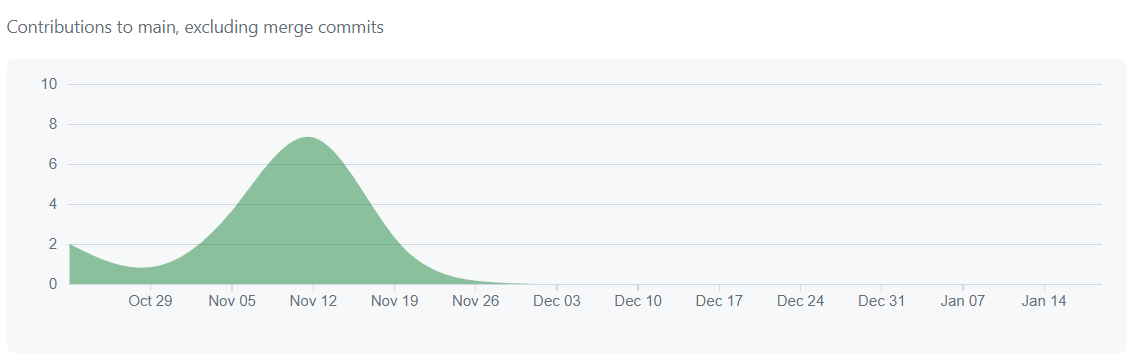
\includegraphics[scale=0.75]{slike/GIT.PNG} %veličina slike u odnosu na originalnu datoteku i pozicija slike
			\centering
			\caption{Dijagram pregleda promjena}
			\label{fig:promjene}
		\end{figure}
		
	